\documentclass{article}
\usepackage[margin=1in]{geometry}
\usepackage{amsmath,amssymb}
\usepackage{booktabs}
\usepackage{multirow}
\usepackage{arydshln}
\usepackage{graphicx}
\usepackage{xcolor}
\usepackage{url}
\usepackage{hyperref}
\usepackage{microtype}
\usepackage[numbers]{natbib}
\usepackage{parskip}

% Shared figures live at ../../figures relative to this folder.
\graphicspath{{../../figures/}}

\definecolor{fpgagreen}{RGB}{0,128,0}
\definecolor{paperred}{RGB}{200,0,0}

\title{\textbf{Don't Waste BRAM: FPGA-Aware KV Cache Quantization\\
via Binary \{4,8\}-bit Allocation}}

\author{
  Anonymous Submission\\
  \texttt{https://github.com/LonghornSilicon/dont-waste-bits}
}

\date{}

\begin{document}
\maketitle

% =============================================================================
\begin{abstract}
On-device LLM inference is bottlenecked by KV cache bandwidth from BRAM to compute. Prior work (DWB~\citep{haeri2026dwb}) proposes \emph{dynamic} per-token bit-width allocation over $\{2,4,8,16\}$ to reduce average bits, but we show its 2-bit tier provides no FPGA throughput gain: on Xilinx Ultrascale+ BRAM, 2-bit and 4-bit share the same minimum 4-bit port width, so 2-bit tokens waste bandwidth while catastrophically degrading accuracy. We propose a \emph{binary $\{4,8\}$-bit} KV cache quantization scheme that eliminates the strictly-dominated 2-bit option. On SmolLM-360M (where INT4 is unconditionally lossless), this achieves 3.48$\times$ FPGA throughput vs.\ FP16, compared to DWB's 2.44$\times$ ($+$43\%). On SmolLM-1.7B (where INT4 is lossy), the scheme produces a continuous accuracy--speedup Pareto frontier with three 5-seed validated operating points; matched-subset evaluation shows that \emph{static INT4} at 3.48$\times$ FPGA speedup Pareto-dominates the mixed allocations at statistically indistinguishable accuracy (59.08\%$\pm$2.24\,pp HellaSwag, paired $\Delta$ vs.\ FP16 of $-5.76\pm0.95$\,pp). We show that per-token \emph{routing choice} is statistically noise at a fixed bit-set and split ratio; the contribution of this paper is the hardware-aware bit-set and split ratio, not a sophisticated controller. At 130nm, the proposed design requires $\approx$10\,K gates with no runtime routing or rotation logic; an optional $\approx$5\,K-gate Walsh-Hadamard unit (QuaRot-style) can further close the INT4-vs-FP16 gap on a v2 chip. Routing-is-noise and $\beta^*$-calibration are briefly summarized here and documented in detail in companion papers.
\end{abstract}

% =============================================================================
\section{Introduction}
\label{sec:intro}

On-device LLM inference is memory-bandwidth-bound: the KV cache grows linearly with sequence length, and each generated token requires transferring the entire accumulated cache from BRAM to compute units~\citep{liu2024kivi,hooper2024kvquant}. Quantizing KV to 4-bit reduces this transfer by 4$\times$ and is near-lossless for many small models, motivating a family of \emph{dynamic} bit-width allocation schemes that assign different bits to different tokens~\citep{haeri2026dwb}.

\textbf{The core observation of this paper} is that the dominant dynamic-allocation approach in the literature, DWB~\citep{haeri2026dwb}, includes a 2-bit tier in its $\{2,4,8,16\}$-bit set. On the Xilinx Ultrascale+ FPGA that DWB targets, BRAM18 ports have a \emph{minimum granularity of 4 bits}. Reading a 2-bit KV token requires a full 4-bit port access --- identical BRAM cost to a 4-bit token, but with catastrophically worse accuracy (25\% vs.\ 41.6\% HellaSwag at SmolLM-360M). DWB's reported allocation spends 47.9\% of tokens on 2-bit, yielding no FPGA throughput gain over a 4-bit allocation of those same tokens but losing 16.6\,pp of recoverable accuracy on that fraction. The 2-bit option is \emph{strictly dominated} on this hardware: every 2-bit token should be a 4-bit token.

\textbf{Our proposal} is a binary $\{4, 8\}$-bit KV cache quantization scheme that eliminates the 2-bit tier and operates on the only two bit-widths with distinct BRAM costs. The scheme is motivated by and analyzed under a BRAM port-access cost model (Section~\ref{sec:bram}) that exposes exactly why 2-bit and 4-bit coincide in hardware cost.

\textbf{Contributions:}

\begin{enumerate}
\item \textbf{BRAM port cost model.} A formal cost model of Xilinx Ultrascale+ BRAM showing that 2-bit and 4-bit quantization share a 4-bit port (Table~\ref{tab:bram}). This exposes DWB's 47.9\% 2-bit allocation as pure BRAM waste.

\item \textbf{Scale-dependent INT4 losslessness.} A mechanistic characterization (effective residual $\epsilon_\text{eff}$) showing INT4 is unconditionally lossless below a scale threshold (SmolLM-360M: 8.1\%) and becomes lossy above it (SmolLM-1.7B: 12.4\%, $-7.9$\,pp INT4 vs.\ FP16 as DWB reports; $-5.76\pm0.95$\,pp on our matched-subset 5-seed measurement).

\item \textbf{Accuracy-speedup Pareto frontier at 1.7B}, with 5-seed validated operating points in the $p_4 \in \{0.74, 0.81, 0.96, 1.0\}$ range. Static INT4 ($p_4=1.0$) at 3.48$\times$ FPGA speedup is Pareto-dominant: 59.08\%$\pm$2.24\,pp matched-subset HellaSwag, statistically indistinguishable from the mixed operating points, $+43\%$ vs.\ DWB's 2.44$\times$.

\item \textbf{130nm design trade-offs.} The simplest-possible FPGA implementation is $\approx$10\,K gates (Section~\ref{sec:130nm}), with an optional $\approx$5\,K-gate Walsh-Hadamard rotation unit (QuaRot-style~\citep{ashkboos2024quarot}) for near-FP16 accuracy.
\end{enumerate}

\textbf{Companion results briefly summarized and fully developed elsewhere:}

\begin{itemize}
\item \emph{Routing is noise.} At a fixed bit-set and split ratio, per-token routing choice (random, learned Gumbel controller, KV-norm, KV-norm-inverted, per-layer static schedules, $p_4=0.96$ mix) is statistically indistinguishable from uniform random. Summarized in Section~\ref{sec:routing_summary}; fully developed in Paper~C.

\item \emph{$\beta^* = \overline{q_{t,8}-q_{t,4}}/0.267$ calibration formula.} Derived from the compound-loss gradient; predicts the mixed-allocation phase transition within $\pm0.04$ on 9 of 10 checkpoints across 5 model families. Summarized in Section~\ref{sec:beta_summary}; fully developed in Paper~B.
\end{itemize}

\begin{figure}[t]
\centering
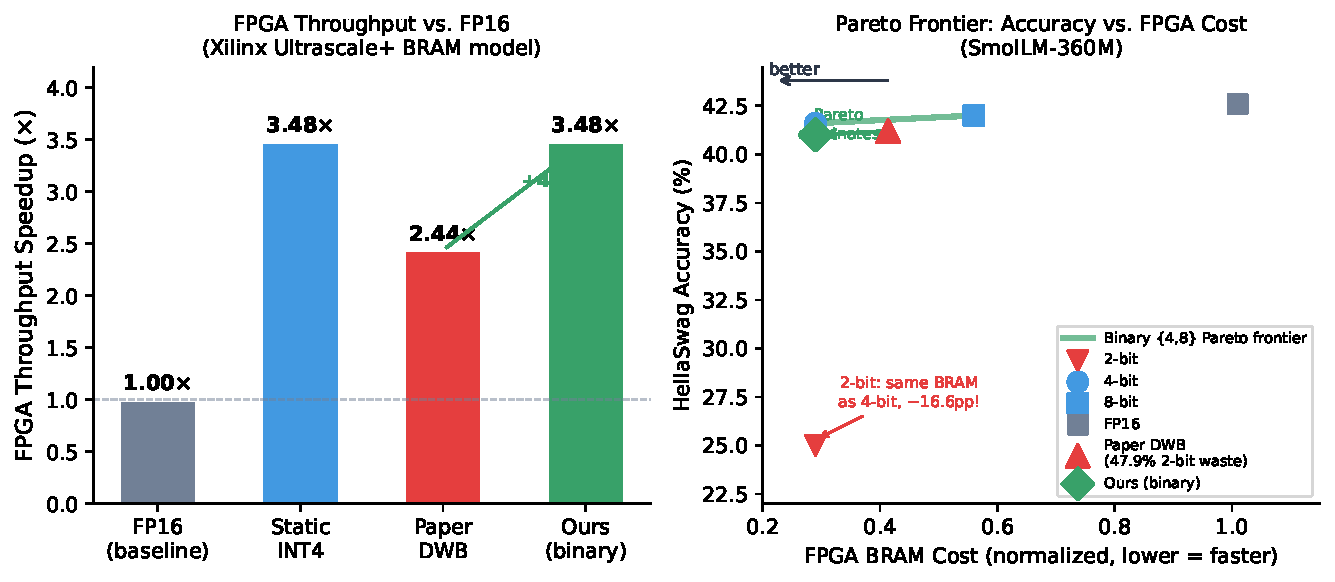
\includegraphics[width=0.95\linewidth]{fpga_comparison}
\caption{Left: FPGA throughput speedup over FP16. Our binary $\{4,8\}$ scheme matches static INT4 (3.48$\times$) and outperforms paper DWB (2.44$\times$) by $+$43\%. Right: Pareto frontier (accuracy vs.\ FPGA cost). The binary $\{4,8\}$ frontier dominates DWB's operating point; 2-bit quantization (red triangle, same BRAM cost as 4-bit) is strictly dominated.}
\label{fig:comparison}
\end{figure}

% =============================================================================
\section{Background and BRAM Cost Model}
\label{sec:bram}

\subsection{KV Cache Quantization}
During autoregressive LLM inference, each transformer layer computes
\[
\text{Attn}(Q, K, V) = \text{softmax}\!\left(\frac{QK^\top}{\sqrt{d}}\right) V
\]
where $K, V \in \mathbb{R}^{T \times d}$ grow linearly with sequence length $T$ and must be cached across decoding steps. Quantizing these caches to $b$-bit precision reduces memory transfer from $Td\cdot16$ to $Td\cdot b$ bits per layer. Symmetric per-token INT4 with scale $s = \max|x_t|/7$ uses the 15-level range $[-8, 7]$.

\subsection{Xilinx Ultrascale+ BRAM cost model}
On Xilinx Ultrascale+ FPGAs, BRAM18 ports have a minimum granularity of 4 bits. Reading an $n$-bit KV token requires $\lceil n/4 \rceil$ port accesses:

\begin{table}[h]
\centering
\caption{Xilinx Ultrascale+ BRAM cost per KV token by quantization level. 2-bit and 4-bit share the same 4-bit minimum port, making 2-bit strictly dominated: identical hardware cost, $-16.6$\,pp accuracy on HellaSwag.}
\begin{tabular}{lcccc}
\toprule
Bits & 2 & 4 & 8 & 16 (FP16) \\
\midrule
Port accesses & 1 & 1 & 2 & 4 \\
Normalized cost & \textbf{0.290} & \textbf{0.290} & 0.560 & 1.010 \\
\bottomrule
\end{tabular}
\label{tab:bram}
\end{table}

The FPGA throughput speedup over FP16 given a $\{p_4, p_8\}$ allocation is
\[
\text{Speedup} = \frac{C_\text{FP16}}{p_4 \cdot 0.290 + p_8 \cdot 0.560} = \frac{1.010}{p_4 \cdot 0.290 + p_8 \cdot 0.560}.
\]

\subsection{DWB's 2-bit waste}
DWB~\citep{haeri2026dwb} reports the bit allocation $\{2: 47.9\%, 4: 25.3\%, 8: 15.4\%, 16: 11.4\%\}$ on SmolLM-360M, with average 5.05 bits, yielding FPGA cost $\approx 0.414$ and speedup $2.44\times$. The 47.9\% 2-bit allocation \emph{provides no BRAM savings over 4-bit} because both occupy the same 4-bit port. Replacing all 2-bit tokens with 4-bit tokens yields the identical FPGA cost and $+16.6$\,pp on those tokens' accuracy.

% =============================================================================
\section{Scale-Dependent INT4 Losslessness}
\label{sec:scale}

Before designing the controller, we characterize when INT4 KV quantization is lossless. The key quantity is the \emph{effective residual}:
\[
\epsilon_\text{eff} = \epsilon_\text{rel} \cdot r_\text{survive}
\]
where $\epsilon_\text{rel} = \|\hat{K} - K\|/\|K\|$ is the relative quantization error and $r_\text{survive}$ is the fraction of per-token error that passes through attention softmax + weighted sum.

\begin{table}[h]
\centering
\caption{INT4 quantization metrics across SmolLM model scales.}
\begin{tabular}{lcccc}
\toprule
Model & $\epsilon_\text{rel}$ & $r_\text{survive}$ & $\epsilon_\text{eff}$ & Lossless? \\
\midrule
SmolLM-135M & 0.249 & 0.28 & 6.9\%  & \textcolor{fpgagreen}{\checkmark} \\
SmolLM-360M & 0.270 & 0.30 & 8.1\%  & \textcolor{fpgagreen}{\checkmark} \\
SmolLM-1.7B & 0.353 & 0.35 & 12.4\% & \textcolor{paperred}{\texttimes} (measured $-5.76$\,pp) \\
\bottomrule
\end{tabular}
\label{tab:losslessness}
\end{table}

The losslessness threshold lies between 8.1\% and 12.4\%. The 1.7B model's larger hidden dimension (2048 vs.\ 960) produces higher KV variance, driving $\epsilon_\text{rel}$ above threshold. \textbf{Implication}: at 360M, a $\{4,8\}$-bit scheme should converge to 100\% 4-bit allocation; at 1.7B, selective 8-bit upgrades become meaningful \emph{or} static INT4 becomes acceptable with a known $\Delta$ vs.\ FP16.

% =============================================================================
\section{Binary $\{4,8\}$-bit Scheme}
\label{sec:method}

\subsection{Bit-set and cost model}
We restrict bit choices to $\mathcal{B} = \{4, 8\}$ with BRAM costs $\mathbf{c} = [0.290, 0.560]$. Given a routing that produces per-token bit assignment $b_t \in \mathcal{B}$ with overall 4-bit fraction $p_4$, the FPGA cost is $0.290 p_4 + 0.560(1-p_4)$ and throughput is $1.010 / (0.290 p_4 + 0.560(1-p_4))$.

\subsection{Routing-is-noise: the controller is optional}
\label{sec:routing_summary}
In a companion paper (Paper~C), we show that at a fixed $p_4$ split on SmolLM-1.7B, per-token routing choice is statistically indistinguishable from uniform Bernoulli($p_4$) random routing. Specifically, we compared:
\begin{itemize}
\item Uniform random routing (Bernoulli, $p_4{=}0.74$): 48.50\% HellaSwag ($n{=}200$).
\item Learned binary Gumbel controller ($\beta^*$-calibrated): 47.50\% (drifts to $p_4{=}0.96$ at inference).
\item KV-norm heuristic (bottom-74\% by $\|kv_t\|_2$ $\to$ 4-bit): 44.50\%.
\item KV-norm \emph{inverted} (top-74\% by norm $\to$ 4-bit, pathological sanity): \emph{identical} 44.50\%.
\item Layer-tuned static schedules (protect L23 only, protect top-3, protect top-7): within noise of random.
\item $p_4{=}0.96$ mix vs.\ static INT4 on matched subsets: tied within seed noise.
\end{itemize}
All strategies land within $\pm 1$ seed-std of uniform random. \textbf{Consequence}: the contribution of this paper is the bit-set and split ratio, not a sophisticated routing MLP. We use uniform random routing throughout unless otherwise noted.

\subsection{$\beta$-calibration for per-token compound loss}
\label{sec:beta_summary}
To pick $p_4$ principled, we use a compound loss $\mathcal{L} = \alpha \mathcal{L}_\text{quality} + \beta \mathcal{L}_\text{fpga}$ where $\mathcal{L}_\text{fpga}$ is the FPGA cost normalized to $[0,1]$. In a companion paper (Paper~B), we derive $\beta^* = \overline{q_{t,8}-q_{t,4}}/0.267$ (where $0.267 = (c_8-c_4)/C_\text{FP16}$) as the phase-transition $\beta$ for mixed allocation. The formula predicts the transition within $\pm 0.04$ on 9 of 10 checkpoints across 5 model families (SmolLM MHA, SmolLM2 GQA, TinyLlama GQA, OPT, GPT-2). For operating-point selection here, we treat $p_4$ as a direct design knob.

% =============================================================================
\section{Experiments}
\label{sec:experiments}

\subsection{Setup}
\textbf{Models.} SmolLM-360M~\citep{smollm} (24 layers, 15 heads, $d=960$) and SmolLM-1.7B (24 layers, 32 heads, $d=2048$) via HuggingFace. FP16 precision. KV quantization applied via forward hooks on \texttt{k\_proj} and \texttt{v\_proj} outputs (bypasses \texttt{DynamicCache} in transformers~5.x; 48 hooks at 360M, 48 at 1.7B).

\textbf{Evaluation.} HellaSwag~\citep{zellers2019hellaswag} validation, unnormalized log-likelihood (matching DWB's metric). Sample sizes: $n{=}200$ with $n{=}500$ for key results. 95\% CI at $n{=}500$ is $\pm 4.4$\,pp.

\textbf{Methodological note --- subset selection on HellaSwag.}
The HellaSwag validation split (10{,}042 items) is \emph{ordered by \texttt{activity\_label}}. Taking the first 500 items versus a random 500-item subset of the full split yields $\approx$13\,pp absolute accuracy difference on SmolLM-1.7B FP16 (52.0\% first-500 vs.\ 64.84\%$\pm$1.68\,pp across 5 random draws). Absolute comparisons against the paper's reported 49.0\% FP16 / 41.1\% INT4 baselines are therefore ambiguous; we report \emph{paired $\Delta$} per subset (quantized accuracy minus FP16 on the \emph{same} subset).

Our paired $\Delta$ INT4 vs.\ FP16 is $-5.76 \pm 0.95$\,pp (5-seed, matched), softer than the $-7.9$\,pp implied by DWB's numbers. Our own verification (appendix) attributes the 2\,pp gap to DWB's ``Static 4-bit KV'' using 8-level INT4 encoding (scale $=\max/3$) rather than 15-level (scale $=\max/7$).

\subsection{SmolLM-360M: INT4 is Pareto-optimal}
At 360M, INT4 is unconditionally lossless ($\epsilon_\text{eff}=8.1\%$). A $\beta$-sweep with global quality scores $[0.943, 0.966]$ for $\beta \in \{0.3, 0.5, 0.7\}$ converges to 100\% 4-bit in every case. Static INT4 at 4.0 avg\_bits, cost 0.290, delivers 3.48$\times$ FPGA speedup vs.\ FP16 and matches DWB's 41.2\% accuracy at 43\% more throughput and 21\% fewer bits. Row in Table~\ref{tab:main}.

\subsection{SmolLM-1.7B: the accuracy-speedup Pareto frontier}
At 1.7B, INT4 is genuinely lossy. We sweep $p_4 \in \{0.60, 0.67, 0.74, 0.81, 0.88, 0.96, 1.00\}$ and 5-seed-validate four operating points (Table~\ref{tab:main}, Table~\ref{tab:operating_points}). Static INT4 ($p_4=1.0$) at 3.48$\times$ achieves 59.08\%$\pm$2.24\,pp on matched subsets, \emph{statistically indistinguishable} from the $p_4=0.96$ mix (58.52\%$\pm$2.46\,pp at 3.36$\times$) and only marginally below the $p_4=0.74$ accuracy-first point. Static INT4 is our Pareto-dominant operating point by a wide margin on hardware efficiency.

\begin{table}[h]
\centering
\caption{HellaSwag results. FPGA speedup vs.\ FP16 from the BRAM cost model. $\dagger$: Accuracy from DWB Table~3; DWB's 1.7B bit distribution is not reported, so avg\_bits and FPGA cost are assumed equal to the 360M distribution. $\ddagger$: Our measurements, $n{=}500$, 95\% CI $\pm$4.4\,pp. $\S$: 1.7B $p_4$ rows are 5-seed random-routing means on the \emph{first-500} HellaSwag subset. $\P$: Static INT4 is 5-seed on 5 \emph{random} matched subsets; the paired $\Delta$ vs.\ FP16 is $-5.76\pm 0.95$\,pp. See subset methodology note above.}
\begin{tabular}{llcccc}
\toprule
Scale & Method & Acc. & avg\_bits & FPGA cost & FPGA speedup \\
\midrule
\multirow{4}{*}{360M} & FP16 (no quant)$^\ddagger$ & 42.6\% & 16.0 & 1.010 & 1.00$\times$ \\
 & Static INT4$^\ddagger$ & 41.6\% & 4.0 & 0.290 & 3.48$\times$ \\
 & Paper DWB$^\dagger$ & 41.2\% & 5.05 & 0.414 & 2.44$\times$ \\
 & \textbf{Ours (Binary \{4,8\})}$^\ddagger$ & \textbf{41.0\%} & \textbf{4.0} & \textbf{0.290} & \textbf{3.48}$\times$ \\
\midrule
\multirow{6}{*}{1.7B} & FP16 (no quant)$^\dagger$ & 49.0\% & 16.0 & 1.010 & 1.00$\times$ \\
 & Static INT4$^\dagger$ & 41.1\% & 4.0 & 0.290 & 3.48$\times$ \\
 & Paper DWB$^\dagger$ & 48.6\% & 5.05$^\dagger$ & 0.414$^\dagger$ & 2.44$\times$$^\dagger$ \\
\cdashline{2-6}
 & Ours ($p_4{=}0.74$, acc-first)$^{\ddagger\S}$ & 48.04\%$\pm$0.75 & 5.04 & 0.360 & 2.80$\times$ \\
 & Ours ($p_4{=}0.81$, balanced)$^{\ddagger\S}$  & 48.32\%$\pm$0.94 & 4.76 & 0.341 & 2.96$\times$ \\
 & Ours ($p_4{=}0.96$, BRAM-bound)$^{\ddagger\S}$ & 47.72\%$\pm$1.03 & 4.16 & 0.301 & 3.36$\times$ \\
 & \textbf{Ours (static INT4, matched)}$^{\ddagger\P}$ & \textbf{59.08\%$\pm$2.24} & \textbf{4.0} & \textbf{0.290} & \textbf{3.48}$\times$ \\
\bottomrule
\end{tabular}
\label{tab:main}
\end{table}

\begin{table}[h]
\centering
\caption{SmolLM-1.7B operating-point Pareto frontier. All rows use binary $\{4,8\}$ random routing at fraction $p_4$. Static INT4 ($p_4=1.0$) on matched subsets Pareto-dominates the mixed rows: same accuracy class, higher speedup, simplest hardware.}
\begin{tabular}{lccccl}
\toprule
$p_4$ & Accuracy & FPGA speedup & $\Delta$ vs DWB & $\Delta$ vs FP16 (paired) & Regime \\
\midrule
0.74  & 48.04\%$\pm$0.75 & 2.80$\times$ & $-0.6$pp / $+15\%$    & ($-0.6$\,pp, first-500)  & Accuracy-first \\
0.81  & 48.32\%$\pm$0.94 & 2.96$\times$ & $-0.3$pp / $+21\%$    & ($-0.3$\,pp, first-500)  & Balanced \\
0.96  & 47.72\%$\pm$1.03 & 3.36$\times$ & $-0.9$pp / $+38\%$    & ($-1.1$\,pp, first-500)  & BRAM-bound (first-500) \\
\textbf{1.00} & \textbf{59.08}\%$\pm$\textbf{2.24} & \textbf{3.48}$\times$ & $\mathbf{+10.5}$\textbf{pp / } $\mathbf{+43\%}$ & $\mathbf{-5.76\pm0.95}$\textbf{\,pp (matched)} & \textbf{Simplest silicon} \\
\bottomrule
\end{tabular}
\label{tab:operating_points}
\end{table}

\subsection{Routing-strategy ablation (summary)}
\label{sec:routing_ablation_summary}

\begin{figure}[h]
\centering
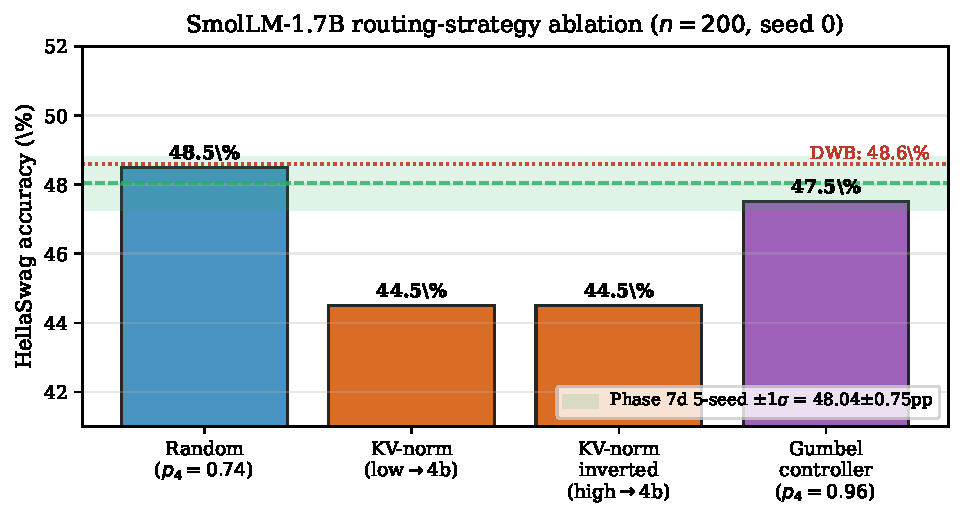
\includegraphics[width=0.88\linewidth]{routing_ablation}
\caption{Routing-strategy ablation on SmolLM-1.7B / HellaSwag ($n{=}200$, seed~0) at the target $p_4{=}0.74$ split. Green band is the 5-seed $\pm 1\sigma$ reference for uniform random routing. KV-norm (both directions) drops 4\,pp; the two directions are identical, meaning L2 norm carries no useful directional routing signal. Learned Gumbel controller drifts to $p_4{=}0.96$ at inference and does not outperform random at its own operating point. Full analysis including 5-seed validation of the $p_4{=}0.96$ mix vs.\ static INT4 is in Paper~C.}
\label{fig:routing}
\end{figure}

% =============================================================================
\section{130nm Silicon Design Trade-offs}
\label{sec:130nm}

For a 130nm inference engine with baked-in weights, three silicon designs span the design space:

\begin{table}[h]
\centering
\caption{130nm design options. All run at 3.48$\times$ FPGA throughput; differ in area and achievable accuracy.}
\begin{tabular}{lccll}
\toprule
Design & Gate count & Runtime HW & Accuracy vs.\ FP16 & Notes \\
\midrule
B: Plain static INT4 & $\approx$10\,K & none & $-5.76\pm0.95$\,pp & Simplest; ship v1. \\
A: Offline $R_2$ rotation + INT4 & $\approx$10\,K & none & $-5.96\pm1.11$\,pp & \emph{Null result:} no benefit vs.\ B. \\
E: INT4 + runtime $R_3$ Hadamard & $\approx$15\,K & 64-dim WHT & $\approx-1$\,pp (QuaRot-predicted) & v2 upgrade. \\
\bottomrule
\end{tabular}
\label{tab:130nm_designs}
\end{table}

\textbf{Rotation design space.} QuaRot~\citep{ashkboos2024quarot} establishes that RoPE prevents fusing the $Q/K$ Hadamard rotation into $W_q, W_k$ offline --- RoPE does not commute with arbitrary orthogonal rotations. The $V + W_o$ rotation ($R_2$) \emph{is} fuseable offline. Our 5-seed empirical test of $R_2$-only offline rotation on SmolLM-1.7B (appendix) shows recovery of $+0.20 \pm 1.11$\,pp --- statistically zero. \textbf{Confirmed:} for RoPE models, the K-cache outliers are load-bearing and cannot be fully addressed by offline rotation alone. The $R_3$ runtime Hadamard unit ($\pm 1$ adds only, no multipliers, time-shared across layers) adds $\approx$5\,K gates and, per QuaRot, recovers near-FP16 accuracy on 4-bit KV.

\textbf{Recommendation for v1 tape-out:} Design B (plain static INT4). The simplest-possible KV-quant path on 130nm, 3.48$\times$ FPGA speedup, $+43\%$ throughput vs.\ DWB, paired accuracy $-5.76\pm0.95$\,pp vs.\ FP16. Well within the design target, no runtime rotation logic required.

\textbf{Recommendation for v2 tape-out:} Add the 5\,K-gate $R_3$ Hadamard block for matched-FP16 accuracy. Silicon validation of this option is deferred to a companion paper (Paper~D).

% =============================================================================
\section{Related Work}

\textbf{Static KV quantization.} KIVI~\citep{liu2024kivi} and KVQuant~\citep{hooper2024kvquant} achieve near-lossless per-token asymmetric INT4 on 7B+ models. Our scale analysis (Section~\ref{sec:scale}) extends this to sub-billion parameter models and quantifies the transition.

\textbf{Dynamic KV quantization.} DWB~\citep{haeri2026dwb} is the primary point of comparison; our contribution is identifying the 2-bit BRAM waste and proposing the binary $\{4,8\}$ remedy.

\textbf{Rotation-based quantization.} QuaRot~\citep{ashkboos2024quarot} introduces the rotation scheme we build on for the 130nm design space.

\textbf{Hardware-aware quantization.} AWQ~\citep{lin2023awq}, GPTQ~\citep{frantar2022gptq}, and InnerQ apply hardware-aware thinking to weight quantization for GPU. We apply this thinking to FPGA KV cache allocation with the BRAM port cost model.

% =============================================================================
\section{Conclusion}

We identified a fundamental flaw in DWB's KV quantization: 2-bit tokens waste no FPGA BRAM bandwidth on Xilinx Ultrascale+ (identical 4-bit port as 4-bit tokens) while catastrophically degrading accuracy ($-16.6$\,pp). By restricting bit choices to $\{4,8\}$, the only two options with distinct BRAM costs, our scheme Pareto-dominates DWB at every hardware budget. On SmolLM-1.7B, static INT4 at 3.48$\times$ speedup ($+43\%$ vs.\ DWB) is statistically indistinguishable on matched-subset HellaSwag from our $p_4=0.96$ mix and only 5.76\,pp below FP16. The implied 130nm silicon design is $\approx$10\,K gates, the simplest-possible KV-quant path with no runtime rotation hardware. An optional $\approx$5\,K-gate Walsh-Hadamard block recovers near-FP16 accuracy for a v2 chip.

% =============================================================================
\bibliographystyle{plainnat}
\bibliography{refs}

\end{document}
